% This must be in the first 5 lines to tell arXiv to use pdfLaTeX, which is strongly recommended.
\pdfoutput=1
% In particular, the hyperref package requires pdfLaTeX in order to break URLs across lines.

\documentclass[11pt]{article}

% Remove the "review" option to generate the final version.
% \usepackage[review]{ACL2023}
\usepackage{ACL2023}

% Standard package includes
\usepackage{times}
\usepackage{latexsym}

% For proper rendering and hyphenation of words containing Latin characters (including in bib files)
\usepackage[T1]{fontenc}
% For Vietnamese characters
% \usepackage[T5]{fontenc}
% See https://www.latex-project.org/help/documentation/encguide.pdf for other character sets

% This assumes your files are encoded as UTF8
\usepackage[utf8]{inputenc}

% This is not strictly necessary, and may be commented out.
% However, it will improve the layout of the manuscript,
% and will typically save some space.
\usepackage{microtype}

% This is also not strictly necessary, and may be commented out.
% However, it will improve the aesthetics of text in
% the typewriter font.
\usepackage{inconsolata}

\usepackage{graphicx}
% \usepackage{subfigure}
\usepackage{subfig}
\usepackage{tabu}
\usepackage{booktabs} % for professional tables
\usepackage{enumitem}
\usepackage{nicefrac}
\usepackage{wrapfig} 
\usepackage{subfig}
\usepackage{xcolor}

\usepackage{pifont} % for dings
\newcommand{\surrogatefeat}{\ding{67}}
\newcommand{\surrogateemb}{\ding{60}}
\newcommand{\clustering}{\ding{166}}

\usepackage{amsmath}
\usepackage{amssymb}
\usepackage{mathtools}
\usepackage{amsthm}
\usepackage{bbm}

\usepackage{algorithm}
\usepackage[noend]{algorithmic}
\usepackage{xcolor}

\newcommand{\theory}[1]{\ensuremath{\mathcal{#1}}}
\newcommand{\facts}[1]{\ensuremath{\mathcal{#1}}}
\newcommand{\rules}[1]{\ensuremath{\mathcal{#1}}}
\newcommand{\goal}[1]{\ensuremath{\mathcal{#1}}}
\newcommand{\algo}{\textsc{Lambada}}
\newcommand{\proved}{\textsc{Proved}}
\newcommand{\disproved}{\textsc{Disproved}}
\newcommand{\unk}{\textsc{Unknown}}
\newcommand{\module}[1]{\emph{#1}}


\newtheorem{theorem}{Theorem}
\newtheorem{proposition}[theorem]{Proposition}
\newtheorem{lemma}[theorem]{Lemma}
\newtheorem{corollary}[theorem]{Corollary}
% \theoremstyle{definition}
\newtheorem{definition}[theorem]{Definition}
\newtheorem{assumption}[theorem]{Assumption}
\newtheorem{observation}[theorem]{Observation}
\newtheorem{example}[theorem]{Example}
% \theoremstyle{remark}
\newtheorem{remark}[theorem]{Remark}

% If the title and author information does not fit in the area allocated, uncomment the following
%
%\setlength\titlebox{<dim>}
%
% and set <dim> to something 5cm or larger.

\title{LAMBADA: Backward Chaining for Automated Reasoning in Natural Language}

% Author information can be set in various styles:
% For several authors from the same institution:
% \author{Author 1 \and ... \and Author n \\
%         Address line \\ ... \\ Address line}
% if the names do not fit well on one line use
%         Author 1 \\ {\bf Author 2} \\ ... \\ {\bf Author n} \\
% For authors from different institutions:
% \author{Author 1 \\ Address line \\  ... \\ Address line
%         \And  ... \And
%         Author n \\ Address line \\ ... \\ Address line}
% To start a seperate ``row'' of authors use \AND, as in
% \author{Author 1 \\ Address line \\  ... \\ Address line
%         \AND
%         Author 2 \\ Address line \\ ... \\ Address line \And
%         Author 3 \\ Address line \\ ... \\ Address line}

\author{Seyed Mehran Kazemi, Najoung Kim, Deepti Bhatia, Xin Xu, Deepak Ramachandran \\
  Google Research \\
  \texttt{\{mehrankazemi, njkim, bhatiad, xxujasime, ramachandrand\}@google.com}}

\begin{document}
\maketitle
\begin{abstract}
Remarkable progress has been made on automated reasoning with knowledge specified as unstructured, natural text, by
using the power of large language models (LMs) coupled with methods such as Chain-of-Thought prompting and Selection-Inference. These techniques search for proofs in the forward direction from axioms to the conclusion, which suffers from a combinatorial explosion of the search space, and thus high failure rates for problems requiring longer chains of reasoning. The classical automated reasoning literature has shown that reasoning in the backward direction (i.e. from the intended conclusion to the set of axioms that support it) is significantly more efficient at proof-finding problems. 
We import this intuition into the LM setting and develop a \emph{Backward Chaining} algorithm, which we call \algo, that decomposes reasoning into four sub-modules, each of which can be simply implemented by few-shot prompted LM inference.
We show that \algo\ achieves massive accuracy boosts over state-of-the-art forward reasoning methods on two challenging logical reasoning datasets, particularly when deep and accurate proof chains are required.
\end{abstract}

\section{Introduction}
Automated reasoning, the ability to draw valid conclusions from explicitly provided knowledge, has been a fundamental goal for AI since its early days \cite{mccarthy1960programs,hewitt1969planner}. While in recent years tremendous progress has been made towards natural language understanding thanks to pre-trained language models (LMs) \cite{brown2020language,chowdhery2022palm}, the performance of these models for logical reasoning still lags behind \cite{rae2021scaling,creswell2022selection} compared to the advancements in other areas such as reading comprehension and question-answering. Yet, logical reasoning---especially logical reasoning with unstructured, natural text---is a fundamental building block for automated knowledge discovery and holds the key for future advances across a variety of scientific domains.

While many problems benefit from LM scaling, scale has been observed to provide limited benefit for solving complex reasoning problems. For example, \citet{creswell2022selection} observed that for the Gopher family of LMs \citep{rae2021scaling}, the scaling law for logic-based tasks is significantly worse than for other language tasks. 
Moreover, while finetuning initially seemed to enable logical reasoning in LMs \cite{clark2020transformers,tafjord2020proofwriter}, further exploration revealed that finetuned LMs mostly exploit spurious correlations 
(e.g., correlation between the number of rules and the final conclusion) 
as opposed to learning to reason \cite{zhang2022paradox,schlegel2022can,liu2022transformers}.
Recently, prompting strategies such as Chain-of-Thought \cite{wei2022chain} and Scratchpad \citep{nye2022show} have found some success for such tasks, although they have been also shown to struggle with proof planning for more complex logical reasoning problems \cite{saparov2022language}.

One solution to the aforementioned problems is to integrate the strength and reliability of classical AI models in logical reasoning with LMs \cite{garcez2020neurosymbolic,marcus2020next}.
In the classic literature, there are two major approaches to logical reasoning \cite{poole2010artificial}: 
\begin{enumerate}[nosep]
    \item \emph{Forward Chaining (FC)} where one starts from the facts and rules (``theory''), and iterates between making new inferences and adding them to the theory until the goal statement can be proved or disproved,
    \item \emph{Backward Chaining (BC)} where one starts from the goal and recursively decomposes it into sub-goals until the sub-goals can be proved or disproved based on the facts.
\end{enumerate}  
Previous approaches to reasoning with LMs mostly incorporate elements of FC into LMs \cite{tafjord2020proofwriter,creswell2022selection}. FC requires selecting a subset of facts and rules from the entire set which might be difficult for an LM as it requires a combinatorial search over a large space. 
Moreover, deciding when to halt and declare failure to prove is challenging in FC \cite{creswell2022selection}, sometimes requiring specialized modules trained on intermediate labels \cite{creswell2022faithful}. Indeed, the classic automated reasoning literature is heavily weighted towards BC or goal-directed  strategies for proof-finding. 

In this paper, we argue and show experimentally that BC is better suited for text-based deductive logical reasoning, as it does not require large combinatorial searches for subset selection and it has more natural halting criteria. We develop a hybrid \textbf{LA}nguage \textbf{M}odel augmented \textbf{BA}ckwar\textbf{D} ch\textbf{A}ining technique, dubbed \emph{\algo}, where BC drives the high-level proof planning, and the LM performs the textual understanding and individual reasoning steps.

We conduct experiments with ProofWriter \cite{tafjord2020proofwriter} and PrOntoQA \cite{saparov2022language} which are challenging datasets for LM reasoning containing examples requiring proof chains of up to $5$ hops in length, and (in the former case) examples where the goal can neither be proved nor disproved from the provided theory. On these datasets, we show that \algo\ has substantially higher deductive accuracy, and is considerably more likely to generate valid reasoning chains compared to other techniques which find correct conclusions with spurious proof traces, while also being more query efficient than other LM-based modular reasoning approaches. Our results strongly indicate that future work on reasoning with LMs should incorporate backward chaining or goal-directed strategies.

\section{Related Work}
The deep learning based models that have been developed to solve text-based (logical) reasoning tasks can be categorized as follows:

\paragraph{Pretraining on relevant tasks:} Pretraining an LM on a corpora relevant to the target reasoning task can lead to improvements \cite{hendrycks2021measuring,shen2021generate}. Pretraining is, however, costly especially for larger LMs. 
\paragraph{Implicit Reasoning:} These approaches typically finetune LMs to produce the desired output directly given the input \cite{clark2020transformers,betz2020critical,saeed2021rulebert,han2022folio}; reasoning happens implicitly in the parameters of the LM.
It has been shown that finetuning LMs on logical reasoning tasks makes them learn spurious correlations \cite{zhang2022paradox,schlegel2022can}, and struggle with multi-hop reasoning \cite{kassner2020pretrained}. Besides, finetuning large LMs is costly and requires a large amount of training data.

\paragraph{Explicit Reasoning:} Recently, approaches that generate the intermediate reasoning steps such as the chain (or tree) of reasoning \cite{wei2022chain,nye2022show,dalvi2021explaining,zelikman2022star,zhang2022improved} have shown massive improvement for many reasoning tasks \cite{suzgun2022challenging}. We compare against a widely successful prompting strategy, named Chain-of-Thought (CoT) \cite{wei2022chain}, from this category. 

\paragraph{Verifiers:} To improve CoT, some works train a verifier using chain-level labels: the verifier takes a reasoning chain produced by the model as input and judges the quality of the chain \cite{cobbe2021training,shen2021generate,jhamtani2020learning,zelikman2022star}. Using this verifier, one can then generate multiple reasoning chains (e.g., by running the algorithm multiple times with different decoding temperatures) and use the best chain according to the verifier. Since \algo\ also generates proofs, verifiers are also applicable to our algorithm. 
In this paper, we assume not having access to chain-level labels, and leave experiments with verifiers as future work.

\paragraph{Length generalization:} A number of approaches specifically look into whether LMs can generalize from examples requiring shorter reasoning chains (shown to them either as demonstration or as finetuning data) to examples requiring longer chains \cite{anil2022exploring,tafjord2020proofwriter}. With our model, length generalization comes for free because the model learns the building blocks of solving the problem that are applied as many times as needed to solve the problem. 

\paragraph{Modular Reasoning:} These approaches break the problem into smaller modules and use separate LMs to solve each module \cite{zhou2022teaching,khot2022decomposed,sprague2022natural,zhou2022least}. 
Most relevant to our work,
in \cite{tafjord2020proofwriter}, a single LM module iteratively and exhaustively derives \emph{all} conclusions based on the facts and rules, and then the goal statement is checked against the final set of conclusions to confirm if it can be proved from the theory. Since exhaustively deriving all conclusions is computationally expensive, \citet{creswell2022selection} consider an alternative approach with two modules: 1- \emph{selection}, which, guided by the goal, selects a subset of the facts and rules from which new conclusions can be derived toward proving the goal, and 2- \emph{inference}, which takes the selected facts and rules and derives a new conclusion. The two modules are called iteratively until a halting criterion is met. In this paper, we compare against the second approach. 

\paragraph{Natural Language Inference (NLI):} Logical reasoning can also be understood as identifying whether a logical entailment relation holds between two propositions (premise and hypothesis; the premise is a set of facts and rules, and the hypothesis is the statement to be proved). In this sense, models trained to perform NLI are also relevant, although inferences under NLI adopt a more relaxed notion of entailment rather than purely logical \cite{dagan2013recognizing,bowman2015large,N18-1101}.

\section{\algo: Language Model Augmented Backward Chaining} \label{sec:method}
In this work, we focus on performing automated reasoning over \emph{facts}, i.e. natural language  assertions such as "Nice people are red", that are coherent but not necessarily grounded in reality. A \emph{rule} is a natural language statement that is either of the form, or can be rewritten in the form, \texttt{``If P then Q''} e.g. \texttt{"Rough, nice people are red"} can be rewritten as  \texttt{"If a person is rough and nice, then they are red"}. \texttt{P} is called the \emph{antecedent} and \texttt{Q} is called the \emph{consequent} of the rule. A \emph{theory} \theory{C} consists of facts $\facts{F}=\{f_1, f_2, \dots, f_n\}$ and rules $\rules{R}=\{r_1, r_2, \dots, r_m\}$. We let \goal{G} represent a \emph{goal} that we would like to prove or disprove based on the facts and rules. 

\begin{example} \label{ex:logic}
Below is an example theory \theory{C} with fictional characters and rules):

\facts{F}=$\{$\texttt{``Fiona is nice'', ``Fiona is rough''}$\}$

\facts{R}=$\{$\texttt{``If someone is smart then they are nice'', ``Rough, nice people are red'', ``Being nice and red implies being round''}$\}$

Based on the above theory, one may want to prove or disprove a goal such as \texttt{``Fiona is red?''}.
\end{example}

\subsection{Backward Chaining}
Backward chaining (BC) is a strategy for reasoning that starts from the goal and recursively breaks the goal into sub-goals based on the rules that can be applied to it, until the sub-goals can be proved or disproved based on the facts or no more rules can be applied to break the sub-goal down further. Whether or not a rule applies to a goal is determined with an operation called \emph{unification} in logic; for the goal \texttt{``Fiona is red?''} in Example~\ref{ex:logic}, for example, the second rule has the same consequent as the goal and so it can be applied, but the other two have different consequences and do not apply. We describe BC with an example.

\begin{example} \label{ex:backward-chain}
Consider the theory and goal in Example~\ref{ex:logic}. BC starts from the goal \texttt{``Fiona is red?''}. First, BC verifies if the goal can be proved or disproved from any of the facts. Since none of the facts prove or disprove the goal, it next verifies if the goal unifies with the consequent of any rule and finds that it unifies with the second rule \texttt{``Rough, nice people are red''}. Therefore, the goal can be broken into two sub-goals: 1- \texttt{``Fiona is rough?''} and 2- \texttt{``Fiona is nice?''}. Since both of these sub-goals can be proved from the facts, BC concludes that the original goal can be proved.
\end{example}

The outcome of BC for a goal is either \proved\ (e.g., for the goal in Example~\ref{ex:backward-chain}), \disproved\ (e.g., for the goal in Example~\ref{ex:backward-chain} if the second rule was \texttt{``Rough, nice people are not red.''}), or \unk\ (e.g., for a goal \texttt{``Fiona is smart?''} in Example~\ref{ex:backward-chain}).

\subsection{LM Modules in \algo}
% We now describe how BC can be combined with LMs to enable text-based logical reasoning. 
To use BC for text-based reasoning, we introduce four LM-based modules: \emph{Fact Check}, \emph{Rule Selection}, \emph{Goal Decomposition}, and \emph{Sign Agreement}. The four modules (and their sub-modules) are implemented by inference to a pretrained LM, where for each one we provide relevant in-context demonstrations to the LM in the prompt (cf. Appendix~\ref{sec:prompts} for the details of the prompts). We start by describing these four modules and then proceed to describing the full algorithm.

\subsubsection{Fact Check} 
Given a set of facts \facts{F} from the theory and a goal \goal{G}, the \module{Fact Check} module verifies if there exists a fact $f\in\facts{F}$ such that $f$ entails \goal{G} (in which case the goal is proved) or $f$ entails the negation of \goal{G} (in which case the goal is disproved). If no such fact can be found, then the truth of \goal{G} remains unknown. 

We implement \module{Fact Check} with two sub-modules: the first sub-module selects a fact from the set of facts that is most relevant to the goal, and the second sub-module verifies if the goal can be proved or disproved based on that fact. 

Since the fact selection sub-module may fail to identify the best fact in the first try, if the truth of the goal remained unknown after one round of calling the sub-modules, the selected fact can be removed and the sub-modules can then be called again; this process can be repeated multiple times. In our experiments, we call the two sub-modules twice. Note that in some datasets, each theory consists of only a single fact---then the fact selection sub-module is not needed. In such cases, we only make a single call to the fact verification module.

\subsubsection{Rule Selection}
Given a set of rules \rules{R} from the theory and a goal \goal{G}, the \module{Rule Selection} module identifies the rules $r\in\rules{R}$ such that the consequent of $r$ unifies with \goal{G}. These rules are then used for decomposing the goal into sub-goals. If no such rule can be identified, then the truth of \goal{G} remains unknown.

As we did for \module{Fact Check}, we implement \module{Rule Selection} with two sub-modules: the first sub-module identifies the consequent of each rule (independent of the goal), and the second sub-module takes the rule consequents and the goal as input and identifies which one unifies with the goal. 
Note that due to the recursive nature of BC, the rule selection module may be invoked multiple times during the proof of a goal. Since identifying the consequent of each rule is independent of the goal, this sub-module only needs to be called once.

\subsubsection{Goal Decomposition}
Given a rule $r$ and a goal \goal{G} such that the consequent of $r$ unifies with \goal{G}, the \module{Goal Decomposition} module identifies the sub-goals that need to be proved in order for $\goal{G}$ to be proved or disproved. The sub-goals are identified based on the antecedent of $r$.

In the case where we succeed in proving the antecedent of $r$, whether the goal is proved or disproved depends on whether the sign of the goal agrees or disagrees with the sign of the consequent of $r$. For instance, in Example~\ref{ex:backward-chain}, for the goal \texttt{``Fiona is red?''}, since the sign of the goal agreed with the sign of the consequent of the second rule and the antecedent of the rule was proved, we concluded that the goal is proved. However, if the second rule was \texttt{``Rough, nice people are not red.''}, then the sign of the goal would disagree with the sign of the consequent and so we would conclude that the goal is disproved. This motivates the fourth module, \module{Sign Agreement}, described next.

\subsubsection{Sign Agreement}
Given a rule $r$ and a goal \goal{G}, the \module{Sign Agreement} module verifies if the sign of the consequent of $r$ agrees or disagrees with the sign of the goal or not.

\begin{algorithm}[t]
\caption{\algo}
\label{algo:back-chain}
\textbf{Input:} Theory: $\theory{C}=(\facts{F}, \rules{R})$, Goal: $\goal{G}$, Max-Depth: D
\begin{algorithmic}[1]
\STATE factCheckResult = \textit{\textcolor{blue}{FactCheck}}(\goal{G}, \facts{F})
\IF{factCheckResult $\neq$ \unk}
    \STATE \textbf{return} factCheckResult
\ENDIF
\IF{D == 0}
    \STATE \textbf{return} \unk
\ENDIF
\STATE $\rules{R}_s$ = \textit{\textcolor{blue}{RuleSelection}}(\goal{G}, \rules{R})
% \STATE \textbf{return} VerifyRules(\theory{C}, Rerank($\rules{R}_s$), \goal{G}, D)
\FOR{$r \in~$Rerank$(\rules{R}_s$)}
    \STATE \textbf{\goal{\mathbf{G}}} = \textit{\textcolor{blue}{GoalDecomposition}}($r, \goal{G}$)
    \IF{ProveSubgoals(\theory{C}, \goal{\mathbf{G}}, D)}
        \IF{\textit{\textcolor{blue}{SignAgreement}}(r, \goal{G})}
            \STATE \textbf{return} \proved
        \ELSE
            \STATE \textbf{return} \disproved
        \ENDIF
    \ENDIF
\ENDFOR    
\STATE \textbf{return} \unk

\end{algorithmic}
\end{algorithm}

\begin{algorithm}[t]
\caption{ProveSubgoals}
\label{algo:prove-sub-goals}
\textbf{Input:} Theory: $\theory{C}=(\facts{F}, \rules{R})$, Sub-Goals: $\goal{\mathbf{G}}$, Max-Depth: D
\begin{algorithmic}[1]
\FOR{\goal{G} in \goal{\mathbf{G}}}
    \STATE result = \algo(\theory{C}, \goal{G}, D-1)
    \IF{result $\neq$ \proved}
        \STATE \textbf{return} False \emph{\# Assuming conjunction}
    \ENDIF
\ENDFOR

\textbf{return} True
\end{algorithmic}
\end{algorithm}

\subsection{The \algo\ Algorithm}
Algorithm~\ref{algo:back-chain} provides a high-level description of how the four LM modules described earlier can be integrated with BC to enable text-based logical reasoning (the function calls corresponding to LM modules are color-coded). 

\algo\ can be understood as a depth-first search algorithm over the facts and the rules. It takes as input a theory $\theory{C}=(\facts{F}, \rules{R})$ containing the facts and rules, a goal \goal{G} that should be proved or disproved based on the theory, and a depth $D$ corresponding to the halting criterion of the algorithm (representing the maximum depth for the search). The search depth is a natural halting criterion corresponding to the maximum number of reasoning hops required for answering questions.

Initially, the algorithm uses the \module{Fact Check} module to check if \goal{G} can be proved or disproved using the facts. If this is the case, then the algorithm stops and returns the result (\proved\ or \disproved). 

If \goal{G} cannot be proved or disproved, then the algorithm checks the depth $D$ to see whether it can continue the search or not. If $D=0$, then the algorithm stops and return \unk\ indicating that \goal{G} could not be proved or disproved. Otherwise, the algorithm proceeds with applying rules.

The algorithm uses the \module{Rule Selection} module to select the rules $\rules{R}_s$ from $\rules{R}$ whose consequent unifies with \goal{G}.
Then for each rule, the algorithm uses the \module{Goal Decomposition} module to decompose \goal{G} into a set of sub-goals $\mathbf{G}$ that need to be proved and checks whether those sub-goals can be proved. If the sub-goals can be proved, then the algorithm uses the \module{Sign Agreement} module to check whether the sign of the rule consequent agrees or disagrees with the sign of \goal{G}. If it does, then the algorithm returns \proved\ and otherwise \disproved. If there is no rule for which the sub-goals can be proved, then \unk\ is returned indicating that \goal{G} cannot be proved or disproved from the theory.

Note that once a set of rules $\rules{R}_s$ are selected, the algorithm proceeds in a depth-first manner (i.e. it exhaustively verifies one rule before going to the next rule). Therefore, if the algorithm can start with the rules that have a higher chance of succeeding at proving or disproving the goal, it can save computations and be less error prone. In this paper, we use a heuristic to rank the rules: we sort them based on their lengths with shorter rules being ranked higher. 
This heuristic is based on the intuition that shorter rules are likely to have fewer sub-goals in their antecedent. We leave more sophisticated ranking strategies as future work.

To verify if $\mathbf{G}$ can be proved or not, here for brevity we assume the rules are in conjunctive form; it is straightforward to extend this to disjunctive form. For each sub-goal, we call \algo\ with the same context, but with the depth $D$ decreased by 1. Given that we assumed a conjunctive form, we return a value of \emph{False} as soon as the algorithm fails to prove one of the sub-goals and \emph{True} if it succeeds in proving all sub-goals.

During a proof, \algo\ may be called multiple times with the same theory and goal; in Appendix~\ref{sec:cache} we explain how cycles and redundant computations can be avoided using a cache.

\begin{figure*}[t]
  \centering
  \subfloat[]{%
  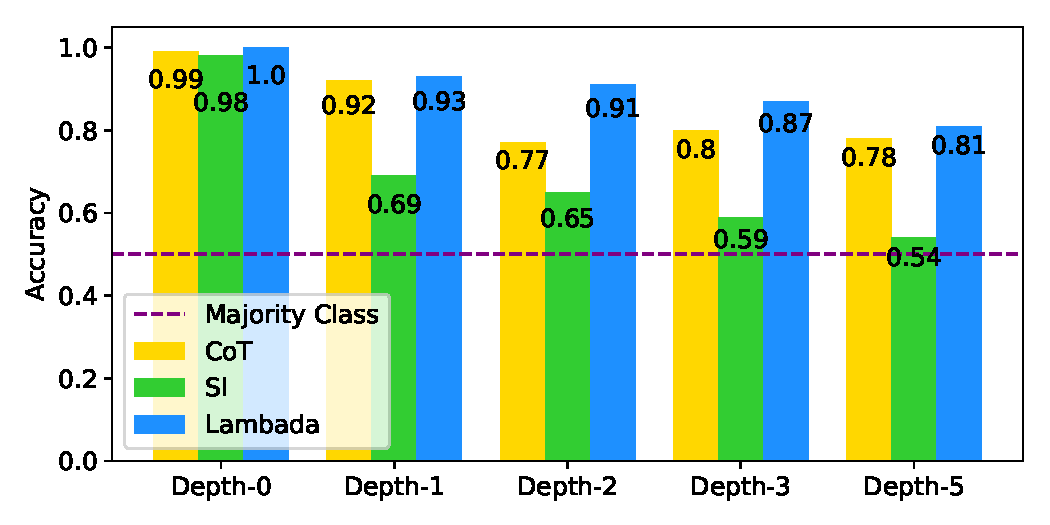
\includegraphics[width=\columnwidth]{proofwriter-tf.pdf}}
~~~~\hspace*{0cm}
  \subfloat[]{%
  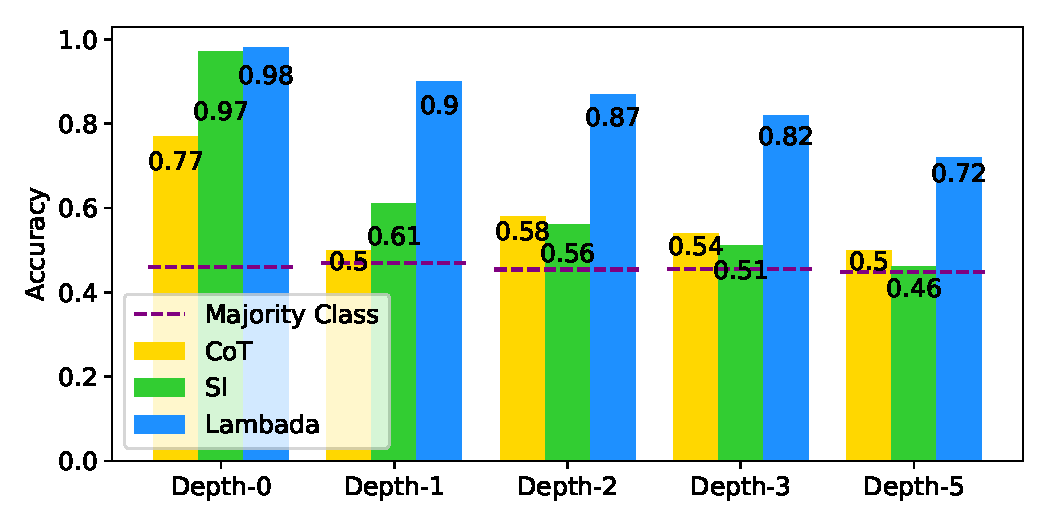
\includegraphics[width=\columnwidth]{proofwriter-tuf.pdf}} %

  \caption{%
  \label{fig:proofwriter} %
  Prediction accuracy results on the (a) ProofWriter-PD and (b) ProofWriter-PUD datasets.}
\end{figure*}

\section{Experimental Setup}
In this section, we describe our baselines and datasets and refer to Appendix~\ref{sec:impl_details} for the implementation details.

\paragraph{Baselines:} We compare against two main baselines for logical reasoning: Chain of Thought (CoT) \cite{wei2022chain}, a state-of-the-art neural reasoning approach based on explicit reasoning, and Selection-Inference (SI) \cite{creswell2022selection}, a state-of-the-art modular reasoning approach.

\paragraph{Datasets:}
We experiment with two challenging logical reasoning datasets:

\textbf{ProofWriter} \cite{tafjord2020proofwriter} is a commonly used synthetic dataset for measuring a model's logical reasoning ability when facts and rules are expressed in naturalistic language form. It contains two subsets: one with open-world assumption (OWA) and another with closed-world assumption (CWA). In this paper, we use the OWA subset. Each example in ProofWriter is a (theory, goal) pair and the label is one of $\{$\proved, \disproved, \unk$\}$ where \unk\ indicates that the goal can neither be proved nor disproved. The dataset is divided into five parts, each part requiring $0$, $\leq 1$, $\leq 2$, $\leq 3$ and $\leq 5$ hops of reasoning, respectively. We report two sets of results on this dataset: 1-with examples labeled \unk\ removed (for fair comparison with previous work), and 2- with all three labels. Note that in this paper, we do not use the proof chains provided in the ProofWriter dataset. For both cases, to reduce overall experimentation cost, we restricted the experiments to the first $1000$ examples in the test set. Hereafter, we refer to the first subset as \emph{ProofWriter-PD} and the second as \emph{ProofWriter-PUD}. 

\textbf{PrOntoQA} \cite{saparov2022language} is a synthetic dataset created to analyze the capacity of LM-based approaches for logical reasoning. Compared to ProofWriter, PrOntoQA has less fact/rule variations; however, the search traces typically contain multiple paths with only one of them leading to the proof, thus enabling testing the proof planning of different models. This dataset has multiple variants; we use the  \emph{fictional characters} version, which is one of the hardest versions accordingn to the results in \cite{saparov2022language}.
Similarly to ProofWriter, each version of PrOntoQA is divided into different parts depending on the number of reasoning hops required ($1$, $3$, and $5$ hops).

\begin{figure}[t]
  \centering
  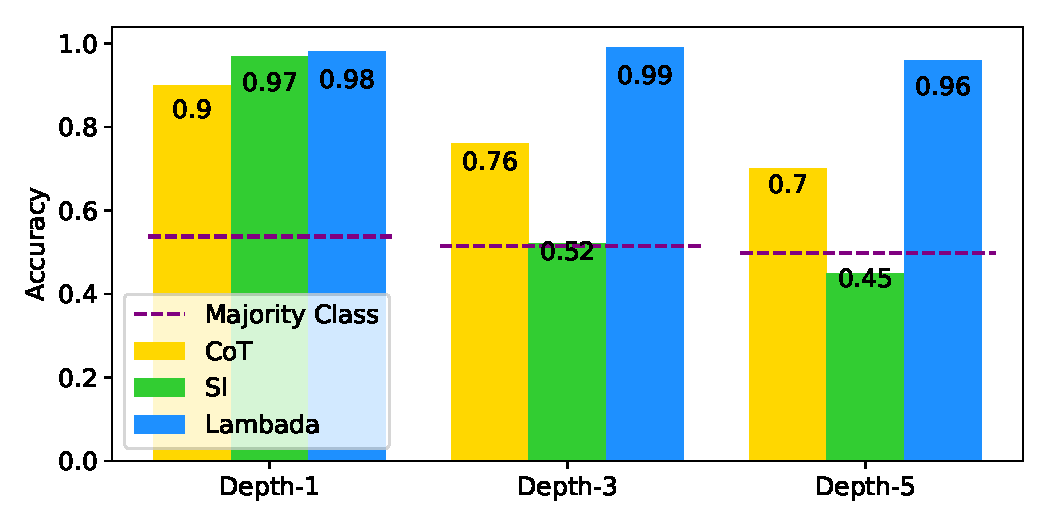
\includegraphics[width=0.9\columnwidth]{prontoqa.pdf}
  \caption{%
  \label{fig:pronto} %
    Prediction accuracy results for \algo\ and the baselines on PrOntoQA.
  }
  \label{fig:pud}
\end{figure}

\section{Experimental Results}
The results for \algo\ and the baselines on the two ProofWriter datasets are provided in Figure~\ref{fig:proofwriter}, and PrOntoQA results are shown in Figure~\ref{fig:pronto}. From the results, we observe that \algo\ significantly outperforms the other two baselines, especially on ProofWriter-PUD which contains \unk\ labels ($44\%$ relative improvement compared to CoT and $56\%$ compared to SI on Depth-5) as well as on the higher depths of PrOntoQA ($37\%$ relative improvement compared to CoT and $113\%$ compared to SI on Depth-5). These results show the merit of \algo\ for logical reasoning and also show that backward chaining (which is the backbone of reasoning in \algo) may be a better choice compared to forward chaining (the backbone in SI). The results also reveal a short-coming of the CoT approach in dealing with \unk\ labels, as, unlike the examples for which the label is \proved\ or \disproved, there is no natural chain of thought for the examples whose labels are \unk.

For higher depths (3+), on the three datasets SI produces predictions that are close to the majority class prediction. We find that it tends to over-predict \disproved\ in the binary case and \unk\ in the three-way classification case (cf. Appendix~\ref{sec:confusion-matrix}), making it perform even worse than the majority class for Depth-5 of PrOntoQA which has more \proved\ labels than \disproved. However, we surprisingly observe that the performance of CoT remains relatively high for the ProofWriter-PD dataset, and the accuracy does not diminish. In the next sub-section, we verify the reason for this behaviour of CoT. 

\subsection{Proof Accuracy}
To understand the reason behind the high accuracy of CoT on higher depths of ProofWriter-PD, we randomly selected $50$ examples from depth-5 of the dataset where CoT predicted the result correctly and manually verified if the proof chain is correct or not. For comparison, we also manually verified the proofs generated by $\algo$ following a similar procedure. 

The results are reported in Figure~\ref{fig:proof_accuracy}. While \algo\ mostly produced correct chains when the predicted label was correct, CoT only generated the correct chain for $28\%$ of the examples. We observe three dominant reasons for the chains being wrong (cf. Appendix~\ref{sec:cot-proof-errors} for examples): 1- hallucinating rules or facts, 2- not understanding conjunction, and 3- making invalid derivations, with hallucination being the main source of error ($48\%$ of the examples). The hallucinated facts and rules mostly resulted in short-cuts to the correct answer. This hints at the possibility of spurious correlations in ProofWriter-PD that can be exploited by CoT. For example, we found that in $9.2\%$ of the examples which require 1+ reasoning hops, the consequent of one of the rules in the theory is the same as the goal to be proved, and for $98.9\%$ of these examples the label is \proved. In several of these examples, CoT simply concluded that the goal can be proved in $0$ hops based on a hallucinated fact. The spurious correlations also explain the fluctuations in the CoT performance across different depths, as the performance depends on how much those correlations appear in the few-shot demonstrations. This result is consistent with previous work that shows when LMs are asked to solve logical reasoning end-to-end, they rely on spurious correlations \cite{zhang2022paradox}. Note that for SI and \algo, the intermediate modules are impervious to the spurious correlations between the input and the label and do not suffer from this issue.

\begin{figure}[t]
  \centering
  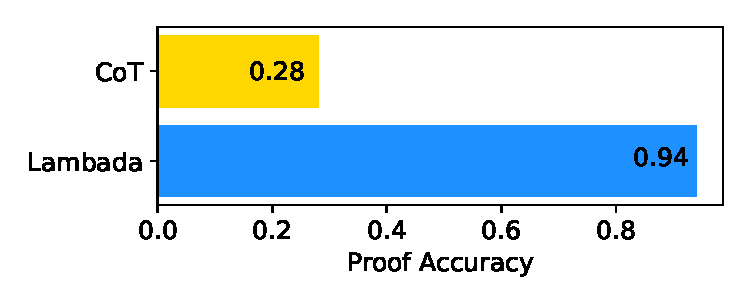
\includegraphics[width=0.8\columnwidth]{proof_accuracy.pdf}
  \caption{%
  \label{fig:proof_accuracy} %
    The proof accuracy of CoT and \algo\ on ProofWriter (Depth-5) for a set of randomly sampled examples for which the models correctly predicted if the goal can be proved or disproved.
  }
  \label{fig:pud}
\end{figure}

\subsection{Individual Module Analysis of \algo} \label{sec:failure-modes}
To understand which components in \algo\ are responsible for the failure cases, we computed the individual accuracy of each of the four modules described in Section~\ref{sec:method} in isolation. For this purpose, we created four datasets from the validation set of the ProofWriter dataset as described below. 

For \module{Fact Check}, we randomly selected 100 examples from the Depth-0 examples. 
For \module{Rule Selection}, we randomly selected 100 examples and manually enumerated every rule whose consequent unifies with the goal. A model prediction is considered correct if it predicts \emph{all} such rules correctly. For \module{Goal Decomposition}, we randomly selected 100 rules and goals such that the consequent of the rule unifies with the goal and then manually wrote the sub-goals. A model prediction is considered correct if it predicts \emph{all} the sub-goals correctly. For \module{Sign Agreement}, we re-used the same examples from the \module{Goal Decomposition} module and manually labeled them with respect to their sign agreement/disagreement.

Based on the results of largest PaLM model in Figure~\ref{fig:component_analysis}, the \module{Rule Selection} module has the lowest accuracy among the different modules followed by the \module{Goal Decomposition}. In the case of \module{Fact Check}, when we allow the model to only select one fact the accuracy is $0.94$ but that increases to a near perfect accuracy when we allow the model to select two facts. The \module{Sign Agreement} module also shows a near perfect accuracy.

The above results show that the \module{Rule Selection} and \module{Goal Decomposition} modules are responsible for the majority of the failure cases. Note that it is possible that the \module{Rule Selection} module fails for some examples but \algo\ still arrives at the correct conclusion and proof. For the theory and goal in Example~\ref{ex:logic}, for example, if there was another rule whose consequent was \texttt{``being red''} and the \module{Rule Selection} module failed to select that rule, \algo\ would still arrive at the correct proof and prediction.

\begin{figure}[t]
  \centering
  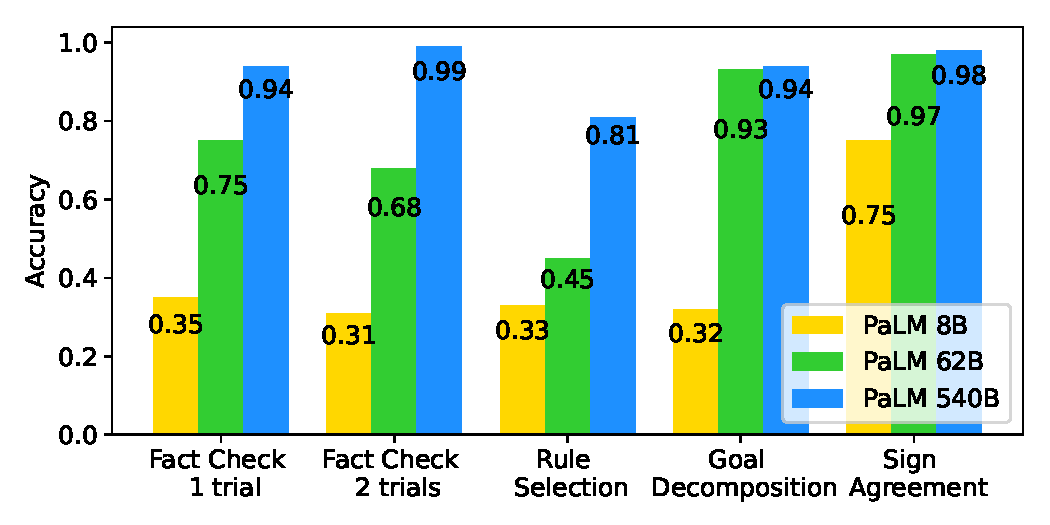
\includegraphics[width=\columnwidth]{component_analysis.pdf}
  \caption{%
  \label{fig:component_analysis} %
    An analysing of the performance of different components in \algo\ in isolation, and for different LM scales.
  }
\end{figure}

\subsection{The role of scale}
We repeat the experiment from Section~\ref{sec:failure-modes} with PaLM 62B and 8B to see the role of LM scale on \algo. 
According to the results in Figure~\ref{fig:component_analysis}, when we use PaLM 62B, the performance of the \module{Goal Decomposition} and \module{Sign Agreement} modules remains comparable, but the performance for the \module{Fact Check} and \module{Rule Selection} modules drops significantly. Unlike the first two modules, the second two modules rely on a one-to-many comparison between the goal and each of the facts/rules which may require a larger model capacity; we believe this is a major reason for the lower performance of PaLM 62B on these two components. Moreoever, we observe that when we switch to PaLM 8B, the results for all components drops significantly, in some cases becoming close to random prediction.

We argue that the extent to which reasoning algorithms break the problem into sub-problem should be dependent on the scale and power of the LMs. If smaller LMs are used, then one may need to break the problem into sub-problems even further (e.g., further decomposing the one-to-many comparisons in the selection module). And as LMs become larger and stronger in the future, one could rely on them to solve problems even with a coarser-grained decomposition of the problem.

\begin{figure}[t]
  \centering
  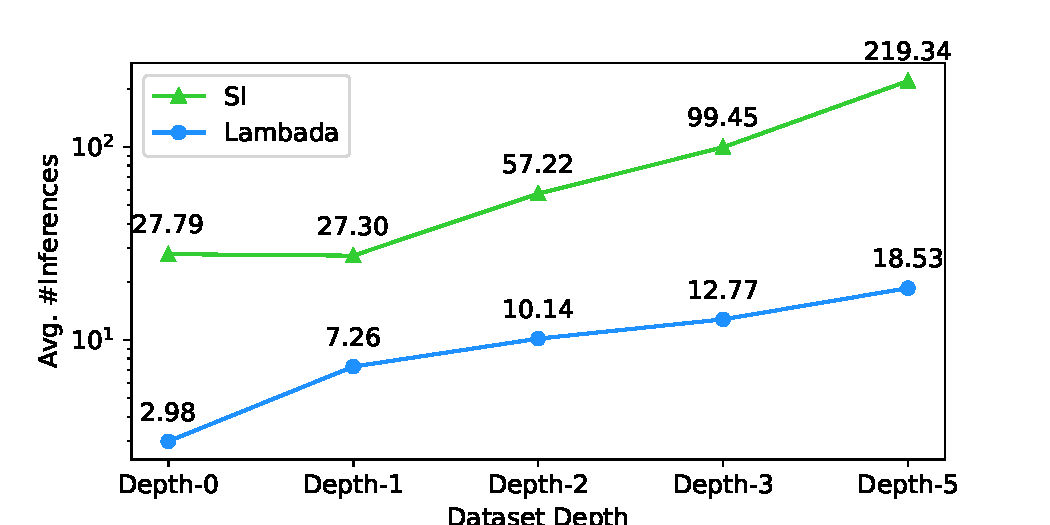
\includegraphics[width=\columnwidth]{call_count.pdf}
  \caption{%
  \label{fig:call_count} %
    Comparing \algo\ and SI with respect to the average number of inference calls they make per example for different subsets of the ProofWriter-PUD dataset.
  }
  \label{fig:pud}
\end{figure}

\subsection{Number of Inference Calls}
\algo\ and SI require multiple LM inference call per example. In Figure~\ref{fig:call_count}, we compare the two models with respect to the average number of inference calls they make to the LM per example, for the different depths of the ProofWriter-PUD dataset. We observe that \algo\ requires significantly fewer inference calls, especially at higher depths. For example, for Depth-1, \algo\ requires 3.8x fewer calls whereas for Depth-5 it requires 11.8x fewer calls.  

\subsection{Qualitative Analysis}
In Figure~\ref{fig:success1}, we show an example of a search trace created by \algo\ where the answer was predicted correctly. 
\algo\ first calls the \module{Fact Check} module; the module specifies that the goal can neither be proved nor disproved. Then \algo\ calls the \module{Rule Selection} module which selects the third rule. The rule is sent to the \module{Goal Decomposition} module which produces the sub-goal \texttt{``Fiona is rough''}. The \module{Fact Check} module cannot prove or disprove the sub-goal, so the \module{Rule Selection} module is called which selects the first and second rules. Starting with the first rule, the \module{Goal Decomposition} module breaks the sub-goal into \texttt{``Fiona is young''}, the \module{Fact Check} module fails to prove or disprove it, and then since the maximum depth reaches \algo\ stops exploring this branch. Then \algo\ considers the second selected rule for which the \module{Goal Decomposition} module produces the sub-goal \module{``Fiona is furry''}. The \module{Fact Check} module specifies that this sub-goal can be proved. Then the \module{Sign Agreement} module is called (not shown on the Figure) to find that for both the rules used on the proof path, the signs agree, and so the goal is proved.

From the figure, one can see how backward chaining helps \algo\ effectively search and create the reasoning chain and how the LM helps in fact checking, rule selection, goal decomposition, and sign agreement checking. In Appendix~\ref{sec:more-results}, we include an example from ProofWriter (Depth-5) that has a much larger search trace.

\begin{figure}[t]
  \centering
  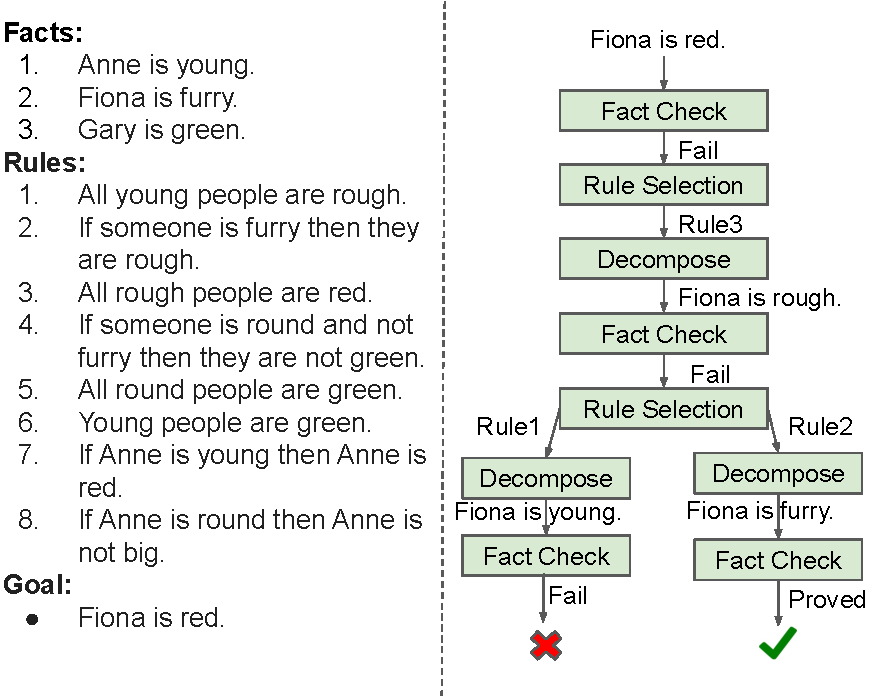
\includegraphics[width=\columnwidth]{success1.pdf}
  \caption{%
  \label{fig:success1} %
    The search trace of \algo\ on an example from ProofWriter with depth=2 where the answer was predicted correctly (the sign agreement module has been omitted for brevity).
  }
\end{figure}

\section{Conclusion}
We developed \algo, an algorithm for text-based deductive logical reasoning that combines the capacity of LMs to handle naturalistic text input with the backward chaining (BC) algorithm for high-level reasoning. We showed that \algo\ achieves significant improvements over competitive existing approaches such as Chain-of-Thought and Selection-Inference both in terms of prediction accuracy (predicting if a statement can be proved or disproved based on a theory) and proof accuracy. Furthermore, we demonstrated how \algo\ efficiently searches the entire proof space to accurately conclude that a statement can neither be proved nor disproved based on the theory. 

Although we only do experiments on formal reasoning problems and datasets, we believe our key insight on the efficacy of goal-directed reasoning with LMs is widely applicable and can be adapted to other NLP tasks where multi-step inference may be required. Going beyond the specific design of \algo\ and its specialized modules, it would be useful to find other BC-inspired methods that might even incorporate BC into the LM directly e.g. a BC version of Chain-of-Thought. 

\bibliography{bib}
\bibliographystyle{acl_natbib}

\appendix

\begin{figure*}[t]
  \centering
  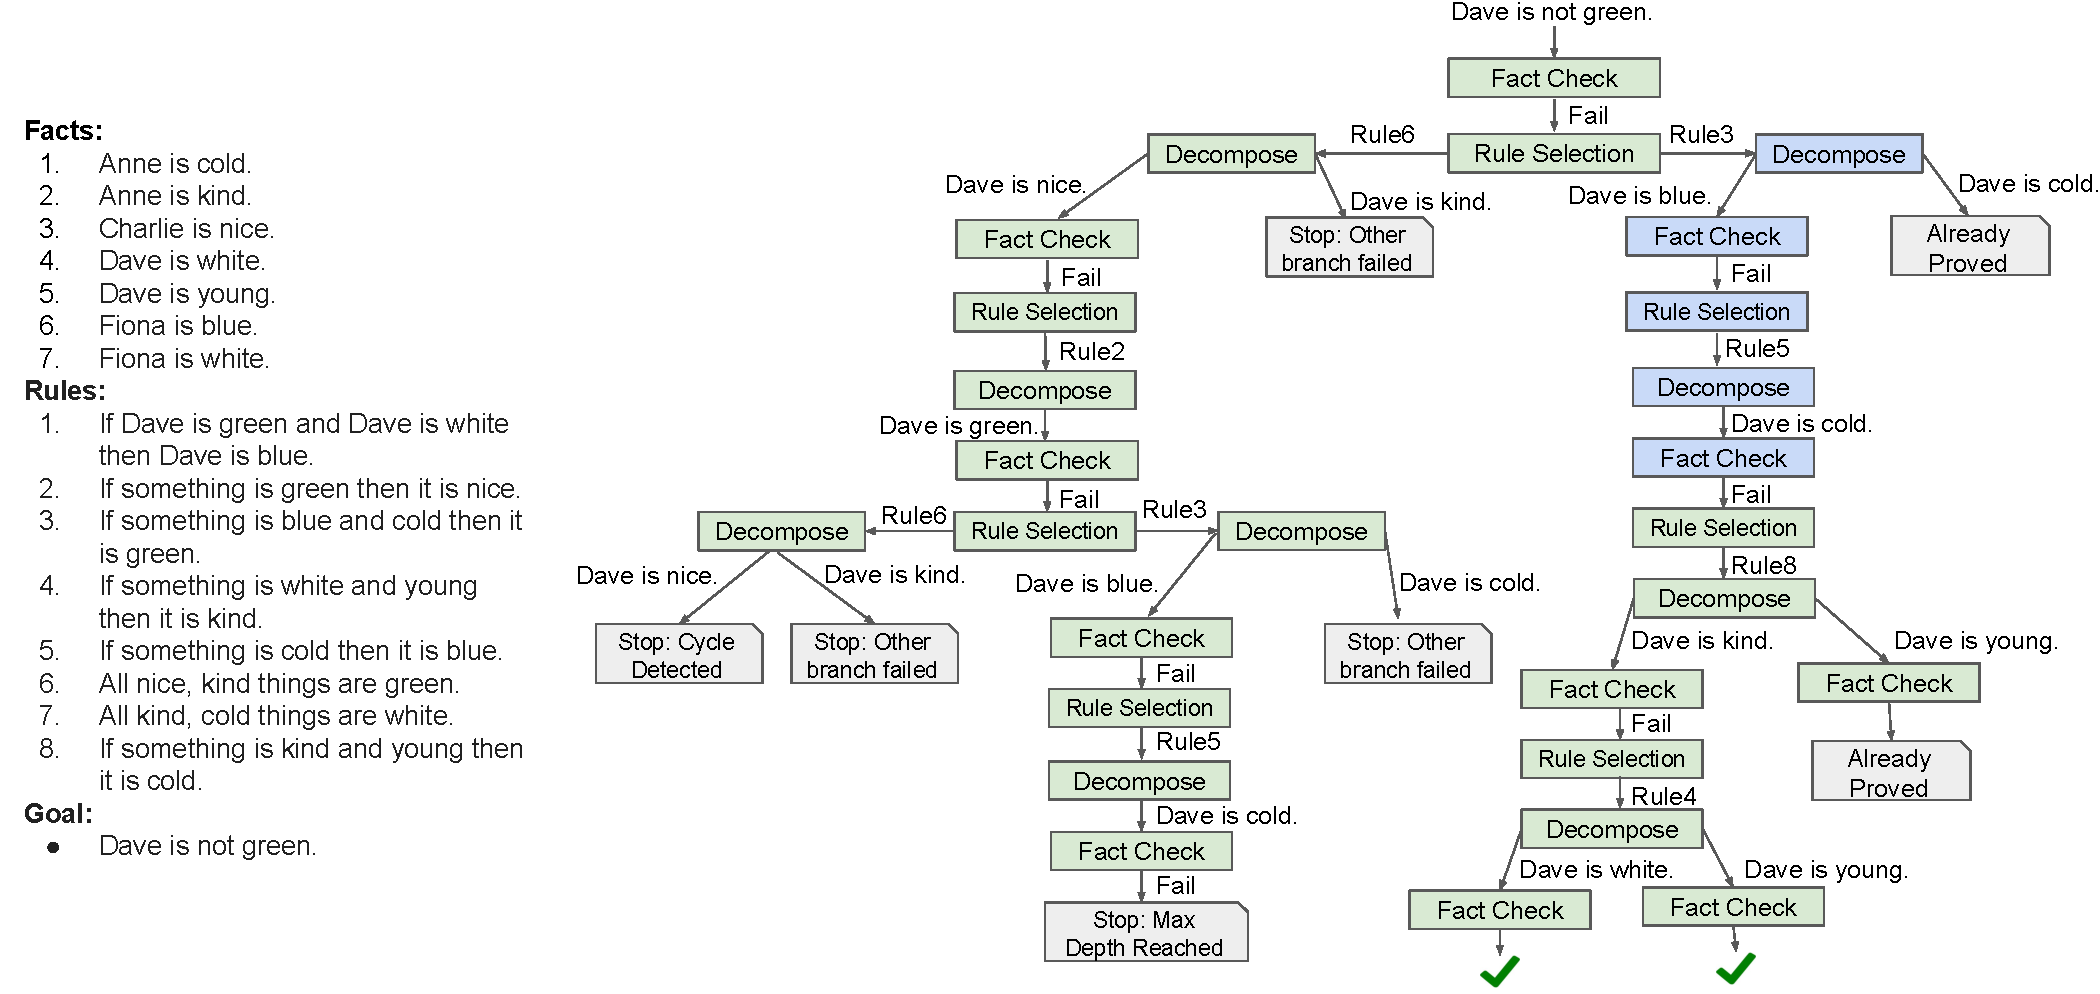
\includegraphics[width=\textwidth]{lambada_depth5_example.pdf}
  \caption{%
  \label{fig:success-depth5} %
    The search trace of \algo\ on an example from ProofWriter with depth=5 where the answer was predicted correctly. The sign agreement module has been omitted for brevity. The modules color-coded with blue represent the calls where the module retrieved the value from the cache instead of calling the LM.
  }
\end{figure*}

\section{Caching and Avoiding Loops for \algo} \label{sec:cache}
Since \algo\ is a recursive algorithm, during the proof of an example Algorithm~\ref{algo:back-chain} may be called with the same goal multiple times. For instance, consider the goal \texttt{``Fiona is round?''} for the theory in Example~\ref{ex:logic}. The goal unifies with the third rule and breaks down to two sub-goals \texttt{``Fiona is nice?''} and \texttt{``Fiona is red?''}. The first sub-goal is then proved with a fact checking. The second sub-goal unifies with the second rule and breaks down to two sub-goals \texttt{``Fiona is rough?''} and  \texttt{``Fiona is nice?''}. The first one can be proved with a fact check; for the second one, since we have already proved this sub-goal, we can save a \module{Fact Check} call if we cache previous results. 

Note that the result of a call to \algo\ can be different depending on the input max depth. For example, the algorithm may return \unk\ when called for the theory and goal in Example~\ref{ex:logic} with max depth 0, and return \proved\ when called with max depth 1. Specifically, if we can prove/disprove a goal at depth $d$, we can conclude that it can be proved/disproved at depths $\geq d$ as well and we can get the value from the cache. Moreover, if the algorithm returns \unk\ for a goal at depth $d$, we can conclude that it will also return \unk\ at depths $<d$. Therefore, if the algorithm is called for a theory and goal at depth $d$, we also check other depths to see if we have the results for other depths that apply to this case. 
Besides having a cache for the entire algorithm that avoids redundant computations when the truth of a goal has been previously computed for a theory, each individual module can also have its own cache as it is possible that the module is called for the same theory and goal. We show one such example in Figure~\ref{fig:success-depth5} (to be discussed in Section~\ref{sec:more-results}).

\algo\ may sometimes run into loops. For example, to prove a (sub-)goal \texttt{``Fiona is round?''}, after recursively identifying rules that unify with it and decomposing it into sub-goals, the algorithm may arrive at a point where it needs to prove the \texttt{``Fiona is round?''} sub-goal, which is equivalent to the initial goal. To avoid such loops, for each path in the proof trace, we keep track of the (sub-)goals that are to be proved and stop further exploring that branch of the search trace when a loop is identified.

Note that in Algorithm~\ref{algo:back-chain}, for clarity of the algorithm we did not include the caching and loop avoidance operations. Also note that caching and loop avoidance mainly help with reducing the number of inference calls.

\section{More Results} \label{sec:more-results}
In this section, we provide some more in-depth qualitative and quantitative analysis of the results from our model and the baselines. 

\subsection{Qualitative Analysis}
In Figure~\ref{fig:success-depth5}, we provide the search trace of \algo\ for an example in ProofWriter (Depth-5) for which \algo\ correctly predicted that the goal is disproved based on the theory. We deliberately selected an example with a large search trace to demonstrate the various aspects of \algo.

\algo\ starts by calling the \module{Fact Check} module on the goal which fails to prove or disprove it. So \module{Rule Selection} is called which identifies two rules that can be applied: Rule3 and Rule6. Since Rule6 is shorter, the reranker ranks it higher; \algo\ starts with this rule and calls the \module{Goal Decomposition} module which breaks the goal into two sub-goals: \texttt{``Dave is nice.''} and \texttt{``Dave is kind.''}. Starting with the first sub-goal, \module{Face Check} fails on it so \module{Rule Selection} is called which selects Rule2 and \module{Goal Decomposition} decomposes the sub-goal into \texttt{``Dave is green.''}. 

Note that if the cycle checking was smart enough to understand that this sub-goal is the negation of the root goal, we could stop further searching this branch. However, we currently only do cycle matching for exact matches so the algorithm continues the search trace.

\module{Fact Check} fails again so \module{Rule Selection} is called which selects Rule3 and Rule6 again, and since Rule6 is shorter the algorithm continues with that rule. \module{Goal Decomposition} breaks the sub-goal into \texttt{``Dave is nice.''} and \texttt{``Dave is kind.''}. Considering the first sub-goal, the algorithm identifies a cycle and stops the search. The second sub-goal is also ignored as there is a conjunction between the sub-goals.

The algorithm then continues with calling \module{Goal Decomposition} for Rule3 which breaks the sub-goal into \texttt{``Dave is blue.''} and \texttt{``Dave is cold.''}. Starting with the first sub-goal, since \module{Fact Check} fails the algorithm calls \module{Rule Selection} which selects Rule5 and \module{Goal Decomposition} breaks the sub-goal into \texttt{``Dave is cold.''}. \module{Face Check} fails on this sub-goal and since maximum depth is reached, the algorithm stops expanding this branch. Moreover, the branch for \texttt{``Dave is cold.''} is no longer pursued because there was a conjunction between the sub-goals and one of them failed.

\begin{figure}[t]
  \centering
  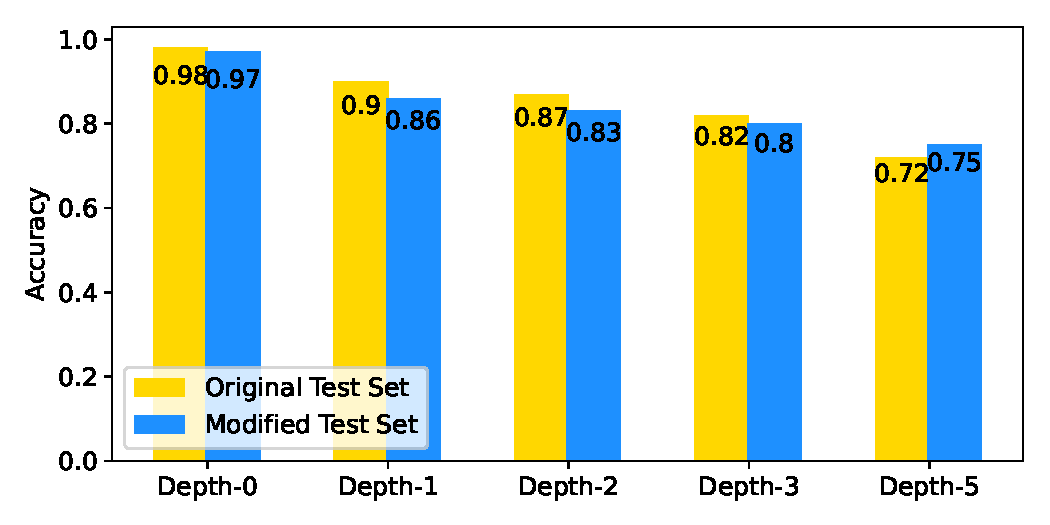
\includegraphics[width=\columnwidth]{sensitivity.pdf}
  \caption{%
  \label{fig:sensitivity} %
    Number of unique inferences generated by SI for Depth-5 of ProofWriter-TF when selection and inference modules are called five times.
  }
\end{figure}

\begin{figure*}[t]
  \centering
  \subfloat[]{%
  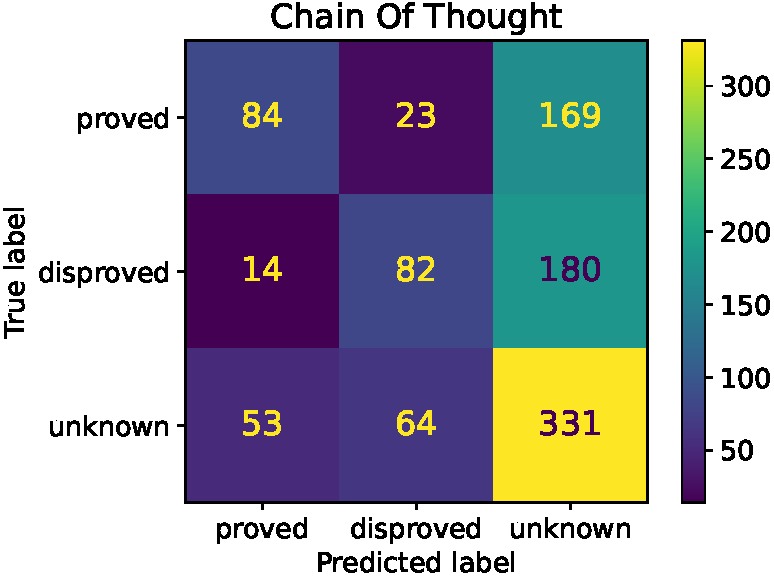
\includegraphics[width=0.33\textwidth]{cot_proofwriter_5_cm.pdf}}
~~~~\hspace*{0cm}
  \subfloat[]{%
  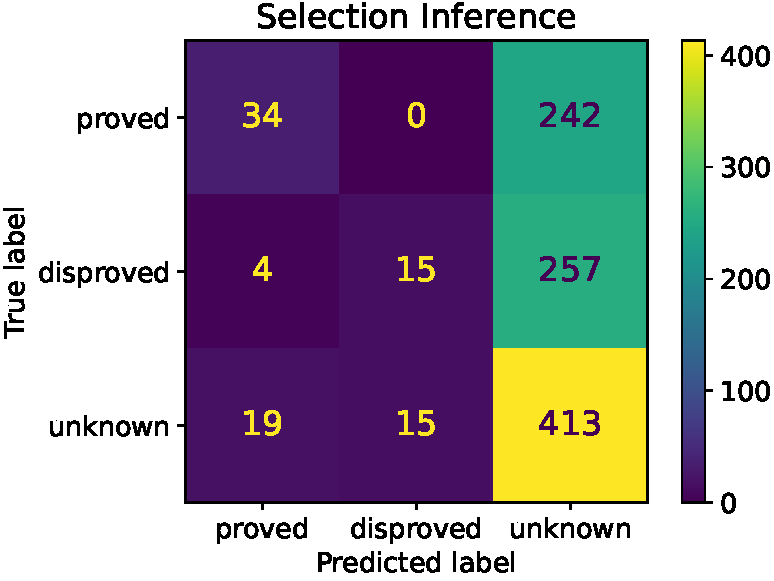
\includegraphics[width=0.33\textwidth]{si_proofwriter_5_cm.pdf}} %
~~~~\hspace*{0cm}
    \subfloat[]{%
  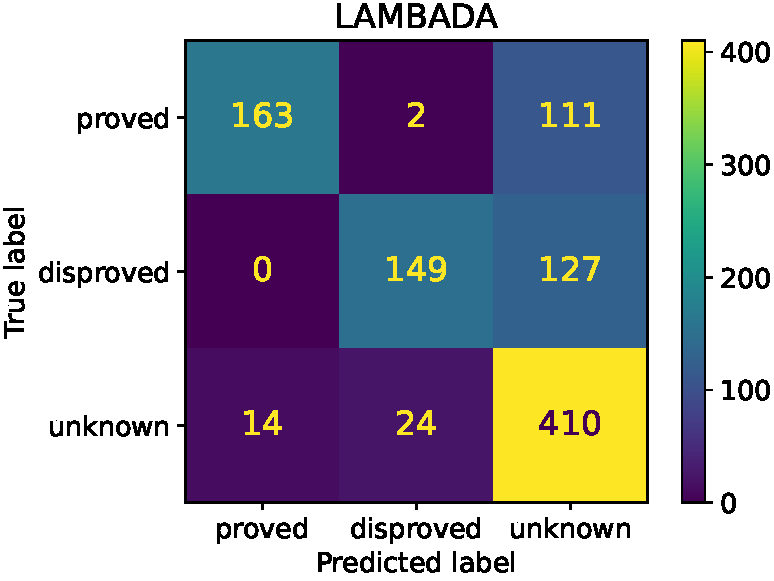
\includegraphics[width=0.33\textwidth]{lambada_proofwriter_5_cm.pdf}} %
  \caption{%
  \label{fig:confusion_matrices} %
  Confusion matrices for (a) CoT, (b) SI, and (c) \algo\ on ProofWriter-PUD (Depth-5).}
\end{figure*}

\begin{figure*}[t]
  \centering
  \subfloat[]{%
  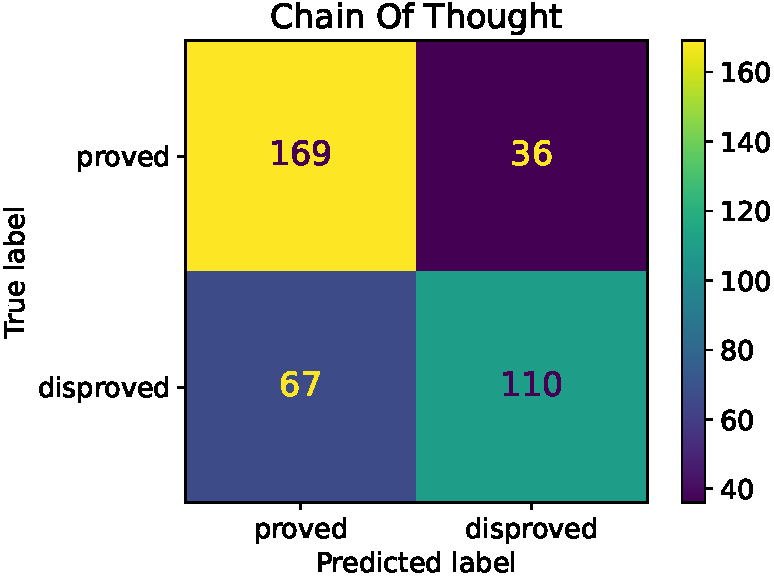
\includegraphics[width=0.33\textwidth]{cot_prontoqa_5_cm.pdf}}
~~~~\hspace*{0cm}
  \subfloat[]{%
  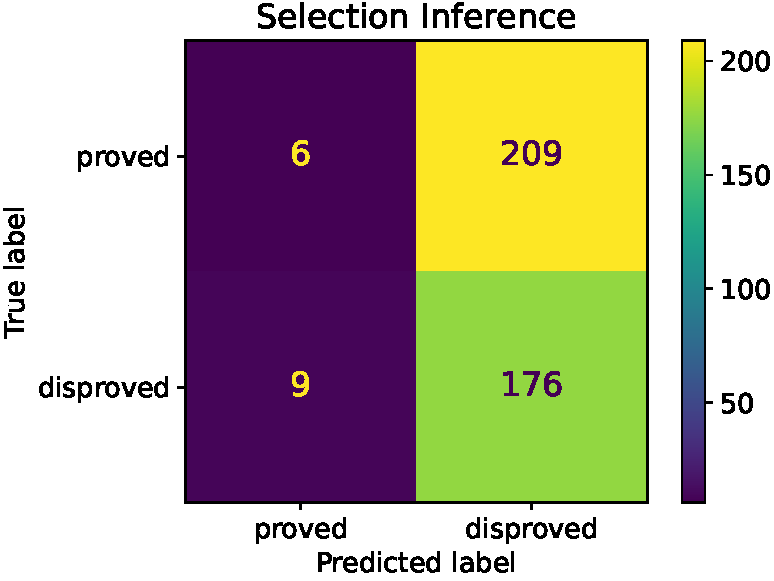
\includegraphics[width=0.33\textwidth]{si_prontoqa_5_cm.pdf}} %
~~~~\hspace*{0cm}
    \subfloat[]{%
  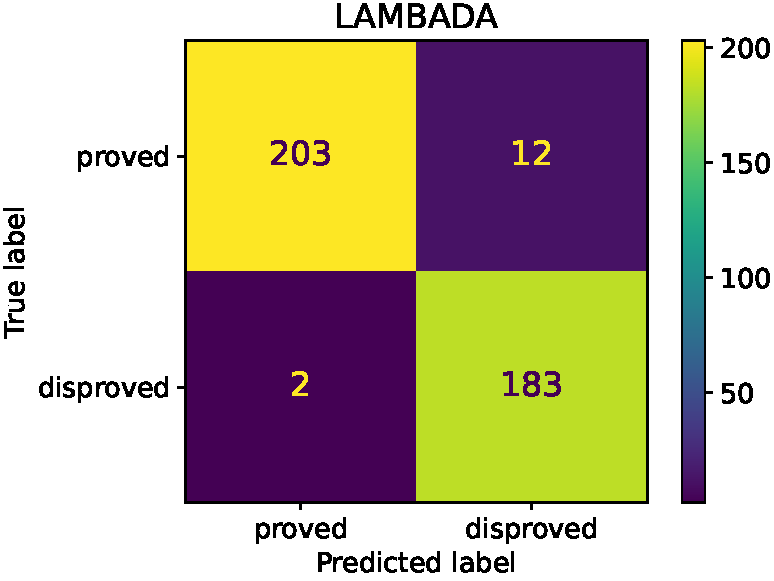
\includegraphics[width=0.33\textwidth]{lambada_prontoqa_5_cm.pdf}} %
  \caption{%
  \label{fig:confusion_pronto} %
  Confusion matrices for (a) CoT, (b) SI, and (c) \algo\ on PrOntoQA (Depth-5).}
\end{figure*}

Moving on to the right branch in Figure~\ref{fig:success-depth5}, the algorithm calls the \module{Goal Decomposition} module for the goal and Rule3. Since we have previously computed it, the sub-goals \texttt{``Dave is blue.''} and \texttt{``Dave is cold.''} are returned from the cache. \module{Fact Check} is called on \texttt{``Dave is blue.''} and since it has been computed before, the result (failuer) is retrieved from the cache. The \module{Rule Selection} module is called, where the result (Rule5) is again retrieved from the cache. \module{Goal Decomposition} is then called and the sub-goal \texttt{``Dave is cold.''} is retrieved from the cache. \module{Fact Check} fails again (retrieved from the cache), \module{Rule Selection} selects Rule8 and \module{Goal Decomposition} produces two sub-goals: \texttt{``Dave is kind.''} and \texttt{``Dave is young.''}. For \texttt{``Dave is kind.''}, \module{Fact Check} fails, \module{Rule Selection} selects Rule4 and \module{Goal Decomposition} produces two sub-goals: \texttt{``Dave is white.''} and \texttt{``Dave is young.''}. For both of these sub-goals, \module{Fact Check} succeeds in proving them. The algorithm then also checks \texttt{``Dave is young.''} for the right branch, but since this sub-goal has already been proved, it just gets the result from the cache.  The algorithm then checks \texttt{``Dave is cold.''} for the rightmost branch, but since this sub-goal has already been proved, it just gets the result from the cache.

The model also calls the \module{Sign Agreement} module for rules on the right branch (not shown on the Figure) and finds out that the sign of the rule and the sub-goals always agrees, except for the very first rule selected (Rule3) so it correctly concludes that the goal is disproved.

\subsection{Sensitivity Analysis} \label{sec:sensitivity}
To analyze the lexical sensitivity of \algo, we created a new test for ProofWriter-PUD which contains tokens that do not appear in demonstration examples. Specifically, we made the following modifications: 1- identified all entity names and mapped each entity name to a new name (previously not appearing in the ProofWriter dataset), 2- identified all animals used in the dataset and mapped each of them to a new animal, 3- identified all adjectives used in the dataset and mapped each of them to a new adjective, and 4- identified all verbs and mapped each verb (except \emph{to be} verbs) to a new verb. Then, using the same few-shot examples as before, we tested the performance of \algo\ on this modified test set and compared the results to the original test set.

The results are presented in Figure~\ref{fig:sensitivity}. According to the results, while we observe some variations in the total accuracy (for some depths the performance going slightly down and for some depths going slightly up), the performance stays in the same ballpark, showing the robustness of \algo. Moreover, comparing the results on the modified test set with those of the baselines reported in the main text, we observe that even on this modified test set, \algo\ performs significantly better than the baselines tested on the original test set.


\subsection{Confusion Matrices} \label{sec:confusion-matrix}
We reported the overall model accuracies in the main text. Here, we report finer-grained confusion matrices that help better understand the biases of the model. Figure~\ref{fig:confusion_matrices} reports the confusion matrices for ProofWriter-PUD (Depth-5) and Figure~\ref{fig:confusion_pronto} reports the confusion matrices for PrOntoQA (Depth-5). According to the results, we observe that whenever \algo\ predicts \proved\ or \disproved, the prediction is most of the times correct. The accuracy is slightly more on cases where the prediction is \proved\ than \disproved. We believe this is because \disproved\ cases typically involve negation that makes the reasoning more complex. However, there are a number of examples for which the label is \proved\ or \disproved, whereas the model predicts \unk.

CoT and SI also show a similar behaviour as \algo\ on ProofWriter-PUD but with a larger bias toward prediction \unk. Moreover, SI shows a large tendency toward predicting \disproved\ for PrOntoQA.

\subsection{CoT Proof Errors} \label{sec:cot-proof-errors}
In the main text, we explained some major categories of errors in CoT proofs even when CoT made the right prediction. In Figure~\ref{fig:cot-failures}, we show failure examples from each category.

\subsection{Duplication Issue in SI}
We find that SI suffers from generating duplicate inferences when the selection and inference modules are ran multiple times. To verify the extent of this issue, we looked at the examples from Depth-5 of ProofWriter-PUD where where SI incorrectly predicted the label to be \unk (these are examples where SI failed to produce good inferences to find a proof). For these examples, we counted the number of unique inferences produced by SI after five rounds. This gives us a notion of how much of the failure is due to generating duplicate inferences. According to the results in Figure~\ref{fig:si-dup}, we see that only for $29\%$ of the examples the inferences are unique; for $7\%$ of the cases all $5$ inferences were the same, and in another $10\%$ of the cases only two unique inferences were made. This shows that SI, and maybe more generally forward chaining approaches, suffer from duplicate inference generation.

\section{Limitations and Future Directions}
We identify two limitations with our current work that can be addressed in future work.

The first limitation is with respect to the applicability to generative cases. The current work is mainly applicable to the logical entailment problems, where one needs to decide if a goal can be proved, disproved, or neither proved nor disproved based on a theory. Future work can extend \algo\ to the generative case where one needs to apply logical reasoning to answer questions such as \texttt{``What color is Fiona?''}.

The second limitation is with respect to the implementation. The calls made to the LM modules in \algo\ are dependent on the value from the previous call. That is, we need to wait for the results from one call before we decide what the next call must be. Since making batch calls to the LMs is typically easier and faster, future work can find ways to implement \algo\ with batch LM calls.

\begin{figure*}[t]
  \centering
  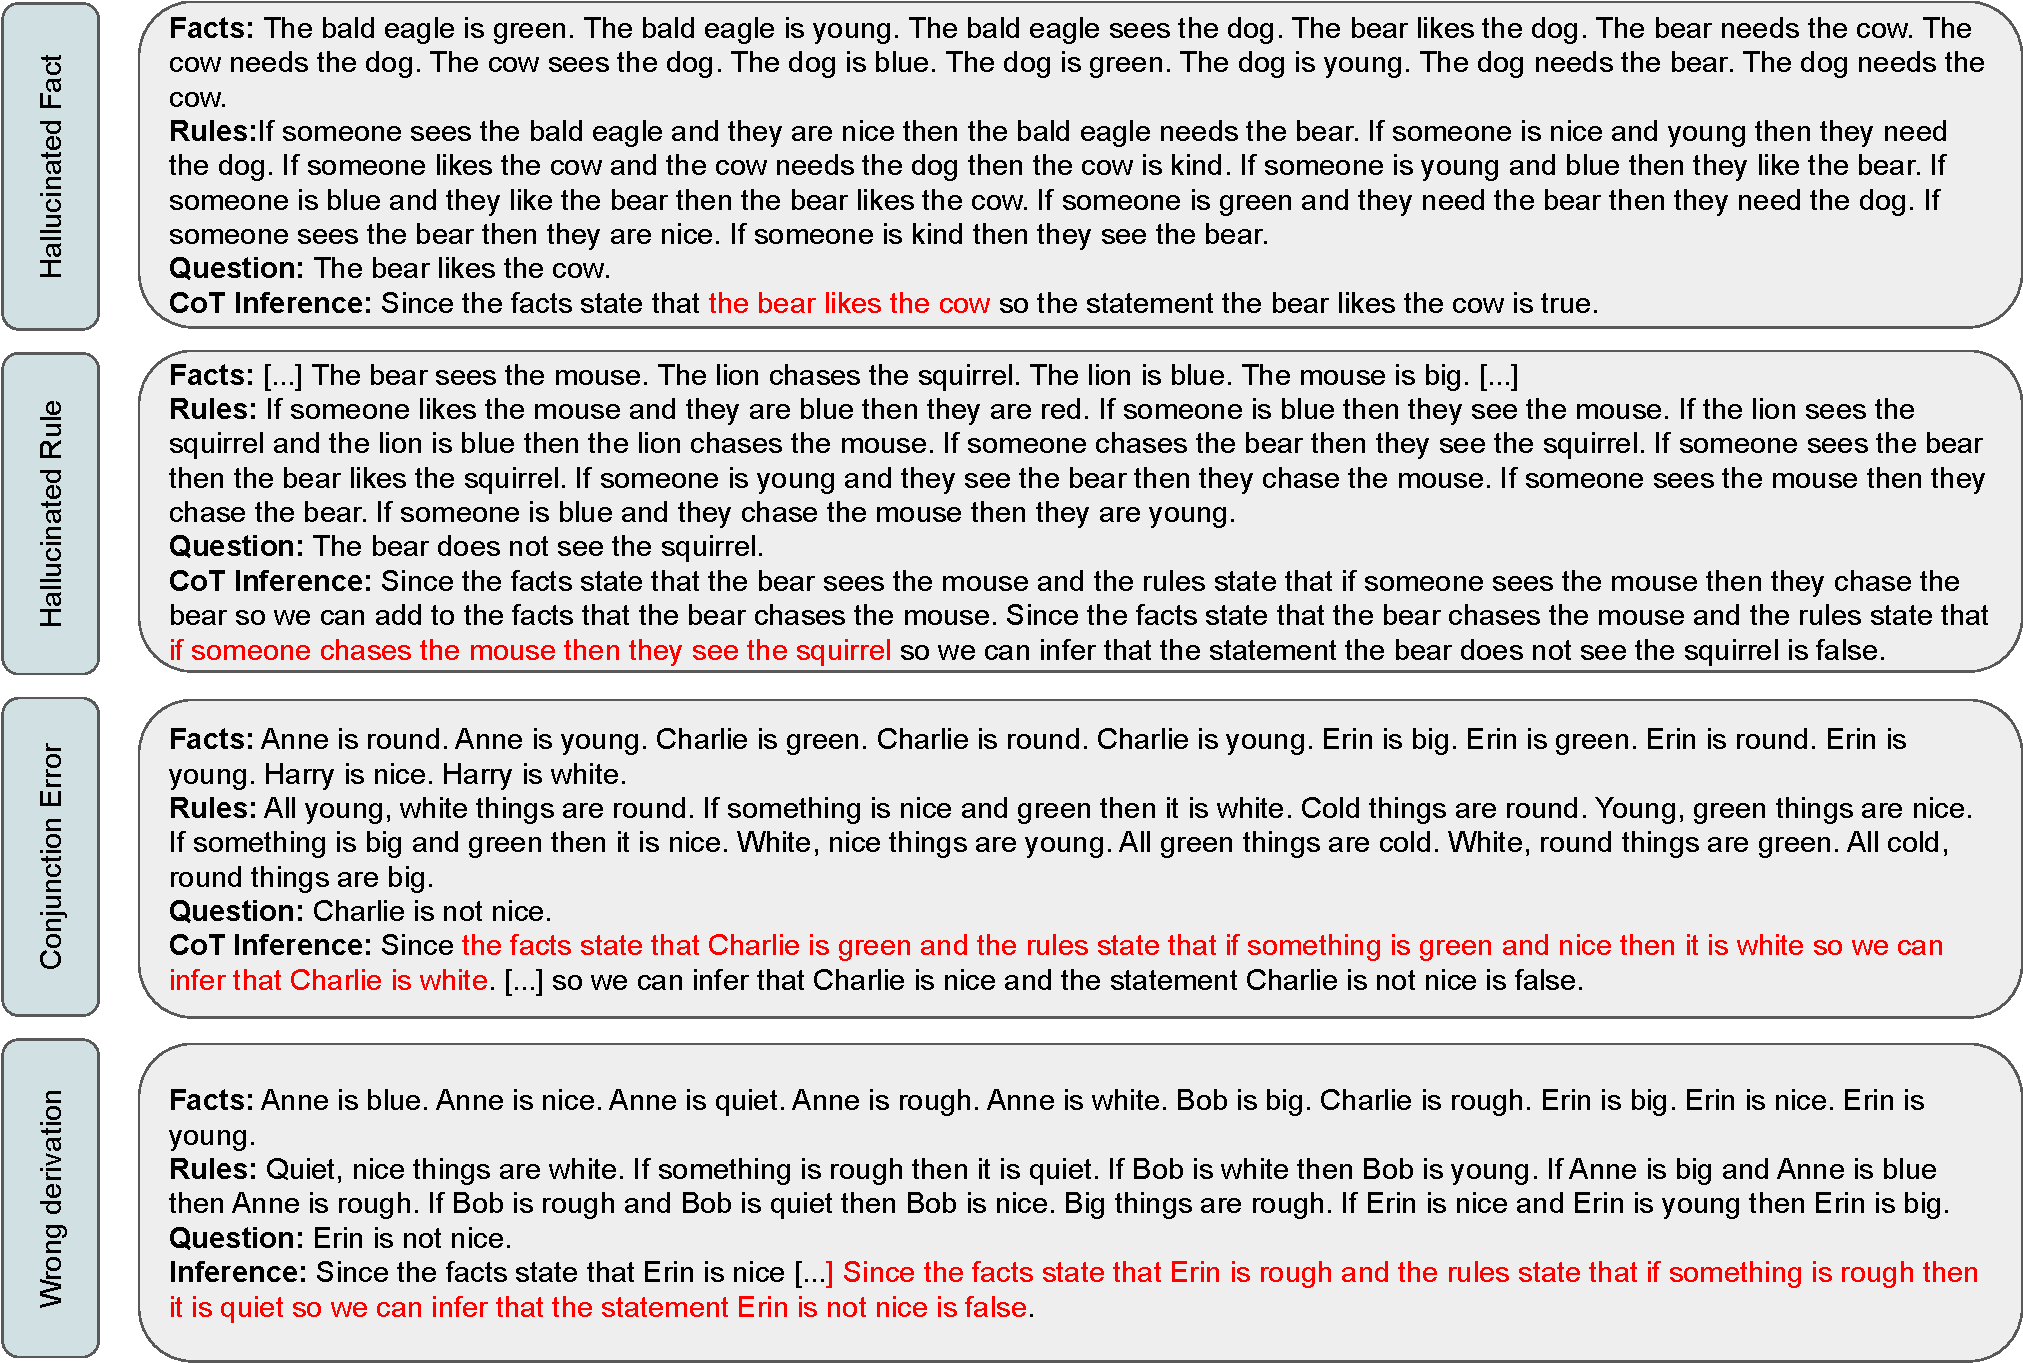
\includegraphics[width=\textwidth]{cot_failure.pdf}
  \caption{%
  \label{fig:cot-failures} %
    Examples of wrong CoT proof chains from four different categories. The erroneous part is marked in red. 
  }
\end{figure*}

\section{Implementation Details} \label{sec:impl_details}
For our experiments, we used the PaLM 540B model \cite{chowdhery2022palm} for all the models (both \algo\ and the baselines). For testing CoT on PrOntoQA, we used the same demonstration examples as the original work but slightly changed the wording by adding conjunctive words such as ``\texttt{Since}'' and ``\texttt{So}'' to make the chains have a better flow. The reason for this modification was that we found when working with PaLM, prompts that have a better flow result in better predictions. This can be viewed from Figure~\ref{fig:cot-prompts} where we compare the performance for the original prompts vs the prompts with the conjunctive words added. It can be viewed that while the latter slightly underperforms on Depth-1 (where the reasoning flow is not as important), it substantially improves the results for higher depths (especially Depth-5). For ProofWriter, we wrote similar few-shot examples. 

For SI, we used the same demonstration examples as in the original work for ProofWriter; for PrOntoQA we wrote few-shot examples following a similar pattern with those for ProofWriter. For each dataset depth we used/wrote specific few-shot examples (e.g., when working with a subset of the data that has examples requiring at most $k$ hops of reasoning, our CoT demonstrations also require only $k$ hops of reasoning), except for ProofWriter Depth-5 where, following the original work, we used it for testing length-generalization and only included examples with chains up to $3$ hops. For running CoT on ProofWriter-PUD, we included extra few-shot examples where the label is \unk; the explanation for these examples is that the goal cannot be proved or disproved with a combination of the facts and the rules. For running SI on ProofWriter-PUD, after obtaining the inferences by running SI, we give the inferences and the goal to our \module{Fact Check} module which decides if the goal can be proved, disproved, or neither. Since \emph{ProofWriter-PD} and \emph{PrOntoQA} are binary datasets but \algo\  makes three-way predictions (\proved, \disproved, and \unk), to test \algo\ on these datasets, similar to SI we combine the \unk\ and \disproved\ predictions into one class.


\begin{figure}[t]
  \centering
  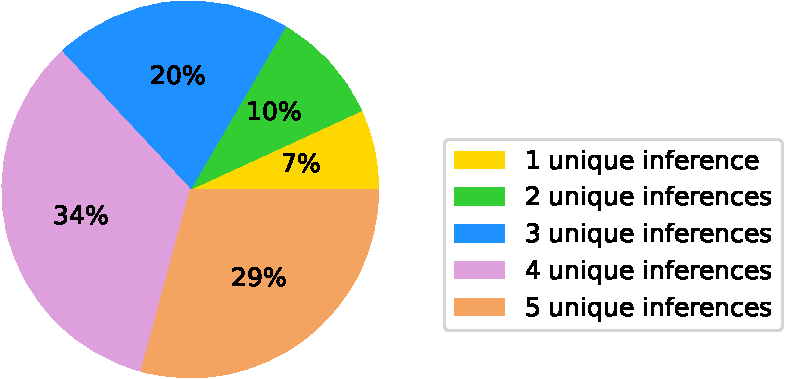
\includegraphics[width=\columnwidth]{si-dup-cropped.pdf}
  \caption{%
  \label{fig:si-dup} %
    Number of unique inferences generated by SI for Depth-5 of ProofWriter-TF when selection and inference modules are called five times.
  }
\end{figure}

\subsection{Prompts}
\label{sec:prompts}
We provide an overview of the prompts we used for each of the four components of our model for the ProofWriter dataset.

For selecting a fact in \module{Fact Check}, our prompt looks like the following:

\indent \texttt{Example 1}\\
\indent \texttt{Fact1: <FACT1> Fact2: <FACT2> ... Factn: <FACTn>}\\
\indent \texttt{Question: <QUESTION>}\\
\indent \texttt{Inference: For the question <QUESTION> the most relevant fact is Facti (<FACTi>).}\\
\indent \texttt{...}\\
\indent \texttt{Example K}\\
\indent \texttt{Fact1: <FACT> Fact2: <FACT> ... Factm: <FACT>}\\
\indent \texttt{Question: <QUESTION>}\\
\indent \texttt{Inference: }

For verifying if the goal/question can be derived from the selected fact, we use the following prompt:

\indent \texttt{Example 1}\\
\indent \texttt{Fact: <FACT>}\\
\indent \texttt{Question: <QUESTION>}\\
\indent \texttt{Inference: The fact <FACT> [X1] the question <QUESTION> so [X2].}\\
\indent \texttt{...}\\
\indent \texttt{Example K}\\
\indent \texttt{Fact: <FACT>}\\
\indent \texttt{Question: <QUESTION>}\\
\indent \texttt{Inference: }\\

In the case where the goal can be proved from the fact, we replace \texttt{[X1]} with \texttt{``is equivalent to''} and \texttt{[X2]} with \texttt{``so the answer is "yes"''}. In the case where the goal can be disproved from the fact, we replace \texttt{[X1]} with \texttt{``is the negation of''} and \texttt{[X2]} with \texttt{``so the answer is "no"''}. And in the case where the goal can neither be proved nor disproved, we replace \texttt{[X1]} with \texttt{``is neither equivalent nor the negation of''} and \texttt{[X2]} with \texttt{``so the question cannot be inferred from the fact''}.

\begin{figure}[t]
  \centering
  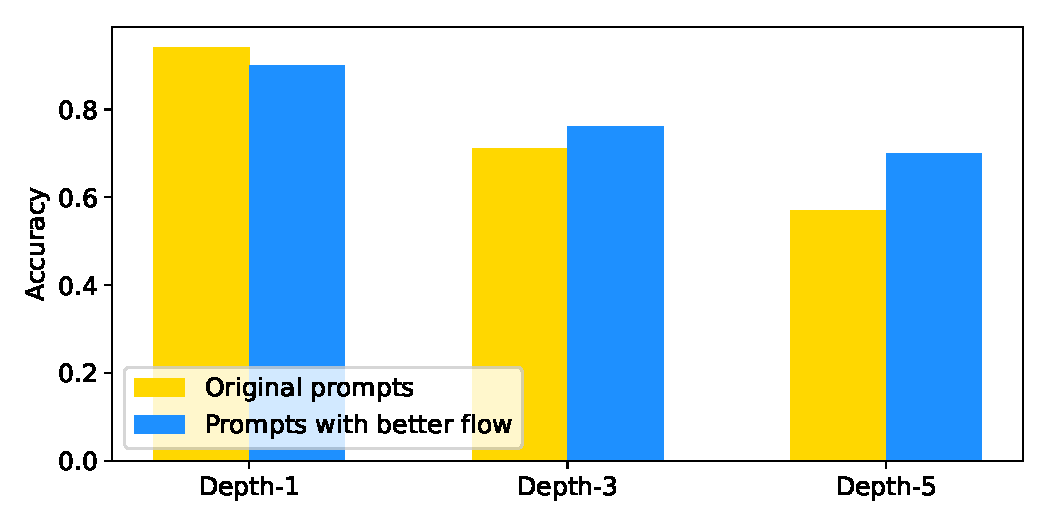
\includegraphics[width=\columnwidth]{cot_prompts.pdf}
  \caption{%
  \label{fig:cot-prompts} %
    CoT results on PrOntoQA with the original prompts vs. the prompts with conjunctive words added to make the sentences flow better.
  }
\end{figure}

For finding the implication/consequent of the rules, we use the following prompt:

\indent \texttt{Example 1}\\
\indent \texttt{Rule1: <RULE1>, Rule2: <RULE2> ... Rulen: <RULEn>}\\
\indent \texttt{Inference: Rule1 implies [X1], $\dots$, Rulen implies [Xn].}\\
\indent \texttt{...}\\
\indent \texttt{Example K}\\
\indent \texttt{Rule1: <RULE1>, Rule2: <RULE2> ... Rulem: <RULEm>}\\
\indent \texttt{Inference: }\\

\texttt{[Xi]}s depend on the consequent of each rule. For rules such as \texttt{``Rough, nice people are red.''} we write \texttt{[Xi]} as \texttt{``(is; red)''}, and for rules such as \texttt{``If the cat chases the dog then the cat sees the dog.''} we write \texttt{[Xi]} as \texttt{``(cat; chase; dog)''}.

For rule selection based on the implications, we use the following prompt:

\indent \texttt{Example 1}\\
\indent \texttt{Rule1 implies <IMLP1>, Rule2 implies <IMPL2>, ..., Rulen implies <IMPLn>}\\
\indent \texttt{Question: <QUESTION>}\\
\indent \texttt{Inference: The question is about <IMPLq>: Rule1 <IMPL1> [X1] <IMPLq>, $\dots$, <IMPLn> [Xn] <IMPLq>.}\\
\indent \texttt{...}\\
\indent \texttt{Example K}\\
\indent \texttt{Rule1 implies <IMLP1>, Rule2 implies <IMPL2>, ..., Rulem implies <IMPLm>}\\
\indent \texttt{Question: <QUESTION>}\\
\indent \texttt{Inference: }\\

where each \texttt{[X1]} is either \texttt{``is applicable to``} or \texttt{``not applicable to``} depending on whether the rule can be applied or not.

For goal decomposition, we use the following prompt:

\indent \texttt{Example 1}\\
\indent \texttt{Rule: <Rule>}\\
\indent \texttt{Question: <QUESTION>}\\
\indent \texttt{Inference: The question subject is <SUBJq> and the rule premises are <PRM>*, so the question breaks down to <SUBQ>*.}\\
\indent \texttt{...}\\
\indent \texttt{Example K}\\
\indent \texttt{Rule: <RULE>}\\
\indent \texttt{Question: <QUESTION>}\\
\indent \texttt{Inference: }\\

where \texttt{<SUBJq>} indicates the subject of the question, \texttt{<PRM>*} indicates the premises/antecedents in the rule (the * indicates that there might be multiple premises), and \texttt{<SUBQ>*} indicates the sub-goals.

Finally, for sign agreement, we use the following prompt:

\indent \texttt{Example 1}\\
\indent \texttt{Rule: <Rule>}\\
\indent \texttt{Question: <QUESTION>}\\
\indent \texttt{Inference: The rule implication <IMLPr> is [Xr], the question <IMPLq> is [Xq], so signs [Xd].}\\
\indent \texttt{...}\\
\indent \texttt{Example K}\\
\indent \texttt{Rule: <RULE>}\\
\indent \texttt{Question: <QUESTION>}\\
\indent \texttt{Inference: }\\

where \texttt{<IMLPr>} shows the implication of the rule and \texttt{<IMPLq>} indicates the implication of the question. \texttt{[Xr]} and \texttt{[Xq]} are either \texttt{``positive``} or \texttt{``negated``} depending on the sign of the implication. \texttt{[Xd]} is either \texttt{``agree``} or \texttt{``disagree``} depending on whether the signs agree or not.

\end{document}
